\documentclass[11pt]{article}
\usepackage{setspace}
\setstretch{1}
\usepackage{amsmath,amssymb, amsthm}
\usepackage{graphicx}
\usepackage{bm}
\usepackage[hang, flushmargin]{footmisc}
\usepackage[colorlinks=true]{hyperref}
\usepackage[nameinlink]{cleveref}
\usepackage{footnotebackref}
\usepackage{url}
\usepackage{listings}
\usepackage[most]{tcolorbox}
\usepackage{inconsolata}
\usepackage[papersize={8.5in,11in}, margin=1in]{geometry}
\usepackage{float}
\usepackage{caption}
\usepackage{esint}
\usepackage{url}
\usepackage{enumitem}
\usepackage{subfig}
\usepackage{wasysym}
\newcommand{\ilc}{\texttt}
\usepackage{etoolbox}
\usepackage{algorithm}
\usepackage{changepage}
% \usepackage{algorithmic}
\usepackage[noend]{algpseudocode}
\usepackage{tikz}
\usetikzlibrary{matrix,positioning,arrows.meta,arrows}
\patchcmd{\thebibliography}{\section*{\refname}}{}{}{}
% \PassOptionsToPackage{hyphens}{url}\usepackage{hyperref}

\providecommand{\myceil}[1]{\left \lceil #1 \right \rceil }
\providecommand{\myfloor}[1]{\left \lfloor #1 \right \rfloor }


\begin{document}



\title{\textbf{MATH 307: Individual Homework 3}}


\author{
Shaochen (Henry) ZHONG, \ilc{sxz517@case.edu}}

\date{Due and submitted on 02/15/2021 \\ Spring 2021, Dr. Guo}
\maketitle

\subsection*{Problem 1}
\textit{Compute all 4th roots of $i$. Express them in polar form and plot them in the complex plane.}\newline

\noindent Known that $i = e ^{i \theta} = e ^{i \frac{\pi}{2}}$, we have its 4th roots being $e^{i (\frac{\theta}{k} + \frac{2j\pi}{k})}$ for $k = 4$ and $j = 0, 1, 2, 3$. So the 4th roots are $e^{i (\frac{\pi}{8} + \frac{j \pi}{2})}$ for $j = 0, 1, 2, 3$. Here's the plotting of these roots where each root is marked in red:


\begin{figure}[H]
    \centering
    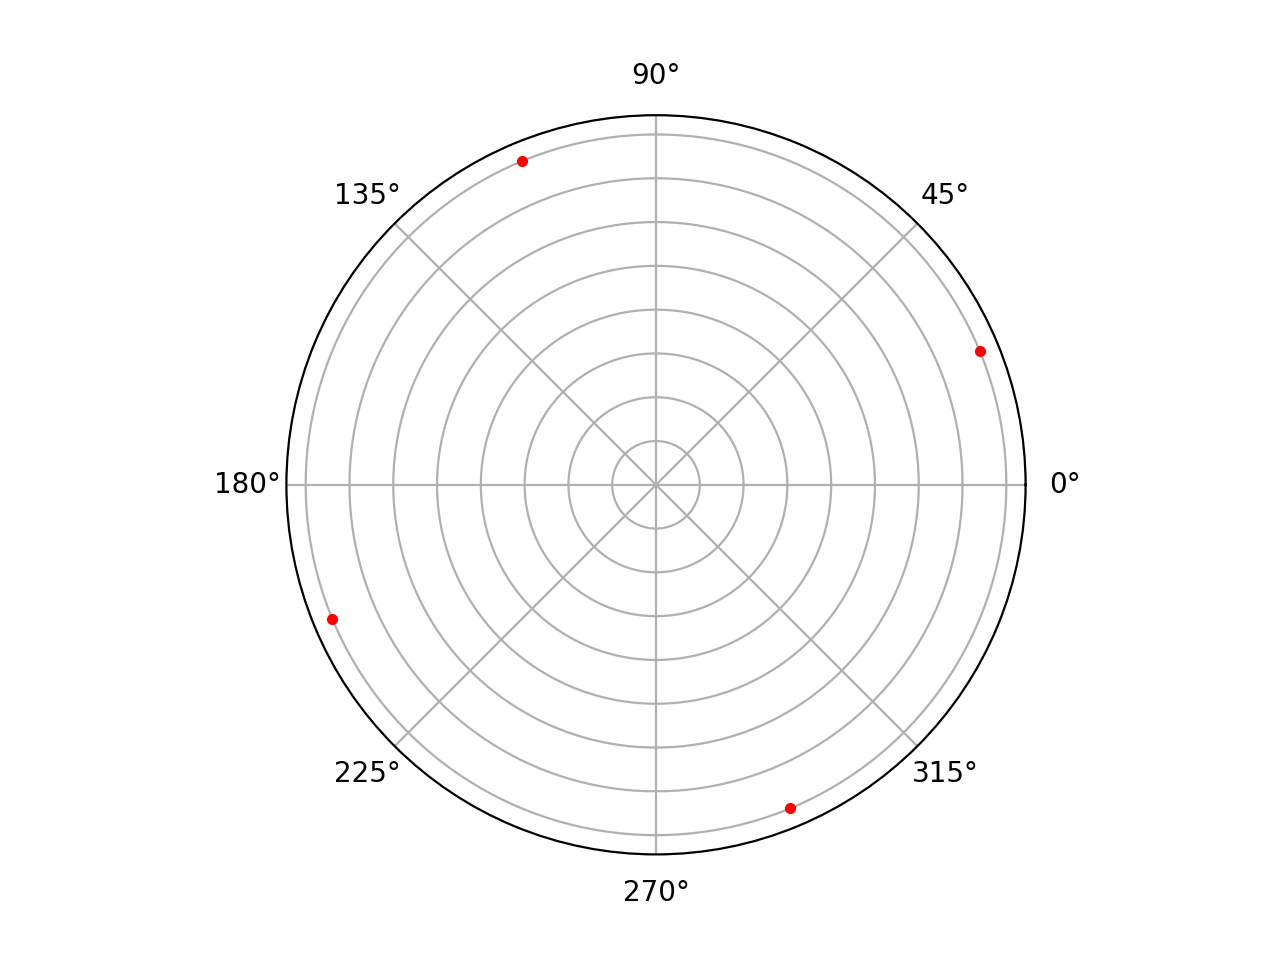
\includegraphics[width=0.5\linewidth]{{fig/fig_p1.png}}
\end{figure}



\subsection*{Problem 2}
\textit{Find the multiplicative inverse of the complex number $z = 2(\cos \pi/3 + i \sin \pi/3)$ and write it in the form $a + ib$.}\newline

\noindent For multiplicative inverse, we must have $z \cdot \frac{1}{z} = 1$.

\begin{align*}
    z &= 2(\cos \pi/3 + i \sin \pi/3) = 2 \cdot e^{\frac{\pi}{3}i} \\
    z^{-1} &= \frac{1}{2} \cdot e^{\frac{-\pi}{3}i} \\
    \Rightarrow &\begin{cases}
        a = \frac{1}{2} \cdot \cos{\frac{-\pi}{3}} = \frac{1}{2} \cdot \frac{1}{2} = \frac{1}{4} \\
        b = \frac{1}{2} \cdot \sin{\frac{-\pi}{3}} = \frac{1}{2} \cdot \frac{-\sqrt{3}}{2} = \frac{-\sqrt{3}}{4}
    \end{cases} \\
    \Longrightarrow z^{-1} &= \frac{1}{4} - \frac{\sqrt{3}}{4}i
\end{align*}


\subsection*{Problem 3}
\textit{Let $z= 1 - i$, find $z^{10}$ using polar representation and write the answer in the form of $a+ib$.}\newline

\noindent To convert to polar form $z = 1 - i = \sqrt{2} e^{\tan^{-1} (\frac{-1}{1})}= \sqrt{2} e^{-\frac{\pi}{4}i}$. Now for $z^{10}$:

\begin{align*}
    z^{10} &= \sqrt{2}^{10} \cdot e^{-\frac{10\pi}{4}i} \\
    &= 32 \cdot e^{-\frac{5\pi}{2}i} \\
    \Rightarrow &\begin{cases}
        a = 32 \cdot \cos{-\frac{5\pi}{2}} = 32 \cdot 0 = 0 \\
        b = 32 \cdot \sin{-\frac{5\pi}{2}} = 32 \cdot -1 = -32
    \end{cases} \\
    \Longrightarrow z^{10} &= 0 -32i = -32i
\end{align*}





\end{document}

